\documentclass[A4]{article}
\usepackage{graphicx}
\usepackage[utf8]{inputenc}
\usepackage[backend=biber, style=iso-numeric, alldates=iso]{biblatex} % bibliografie
\usepackage[autostyle=true,czech=quotes]{csquotes}
\usepackage[czech]{babel}

\addbibresource{bibliography.bib}

\title{Analýza sítě Gnutella}
\author{Lukáš Moravec}
\date{\today}

\begin{document}

\begin{titlepage}
    \maketitle
\end{titlepage}
    
\section{Popis datové sady}
\cite{dataset} Datová sada byla získána ze \cite{snapnets} Standfordské velké kolekce datasetů. Jedná se P2P\footnote{Peer to peer}
síť pro sdílení souborů. Samotná datová sada obsahuje 8717 uzlů a 31525 orientovaných hran. Každý uzel reprezentuje účastníka připojeného
do sítě Gnutella a hrany reprezentují spojení mezi účastníky. Její kompletní znázornění lze vidět na obrázku \ref{network:full}.

\begin{figure}
    \centering
    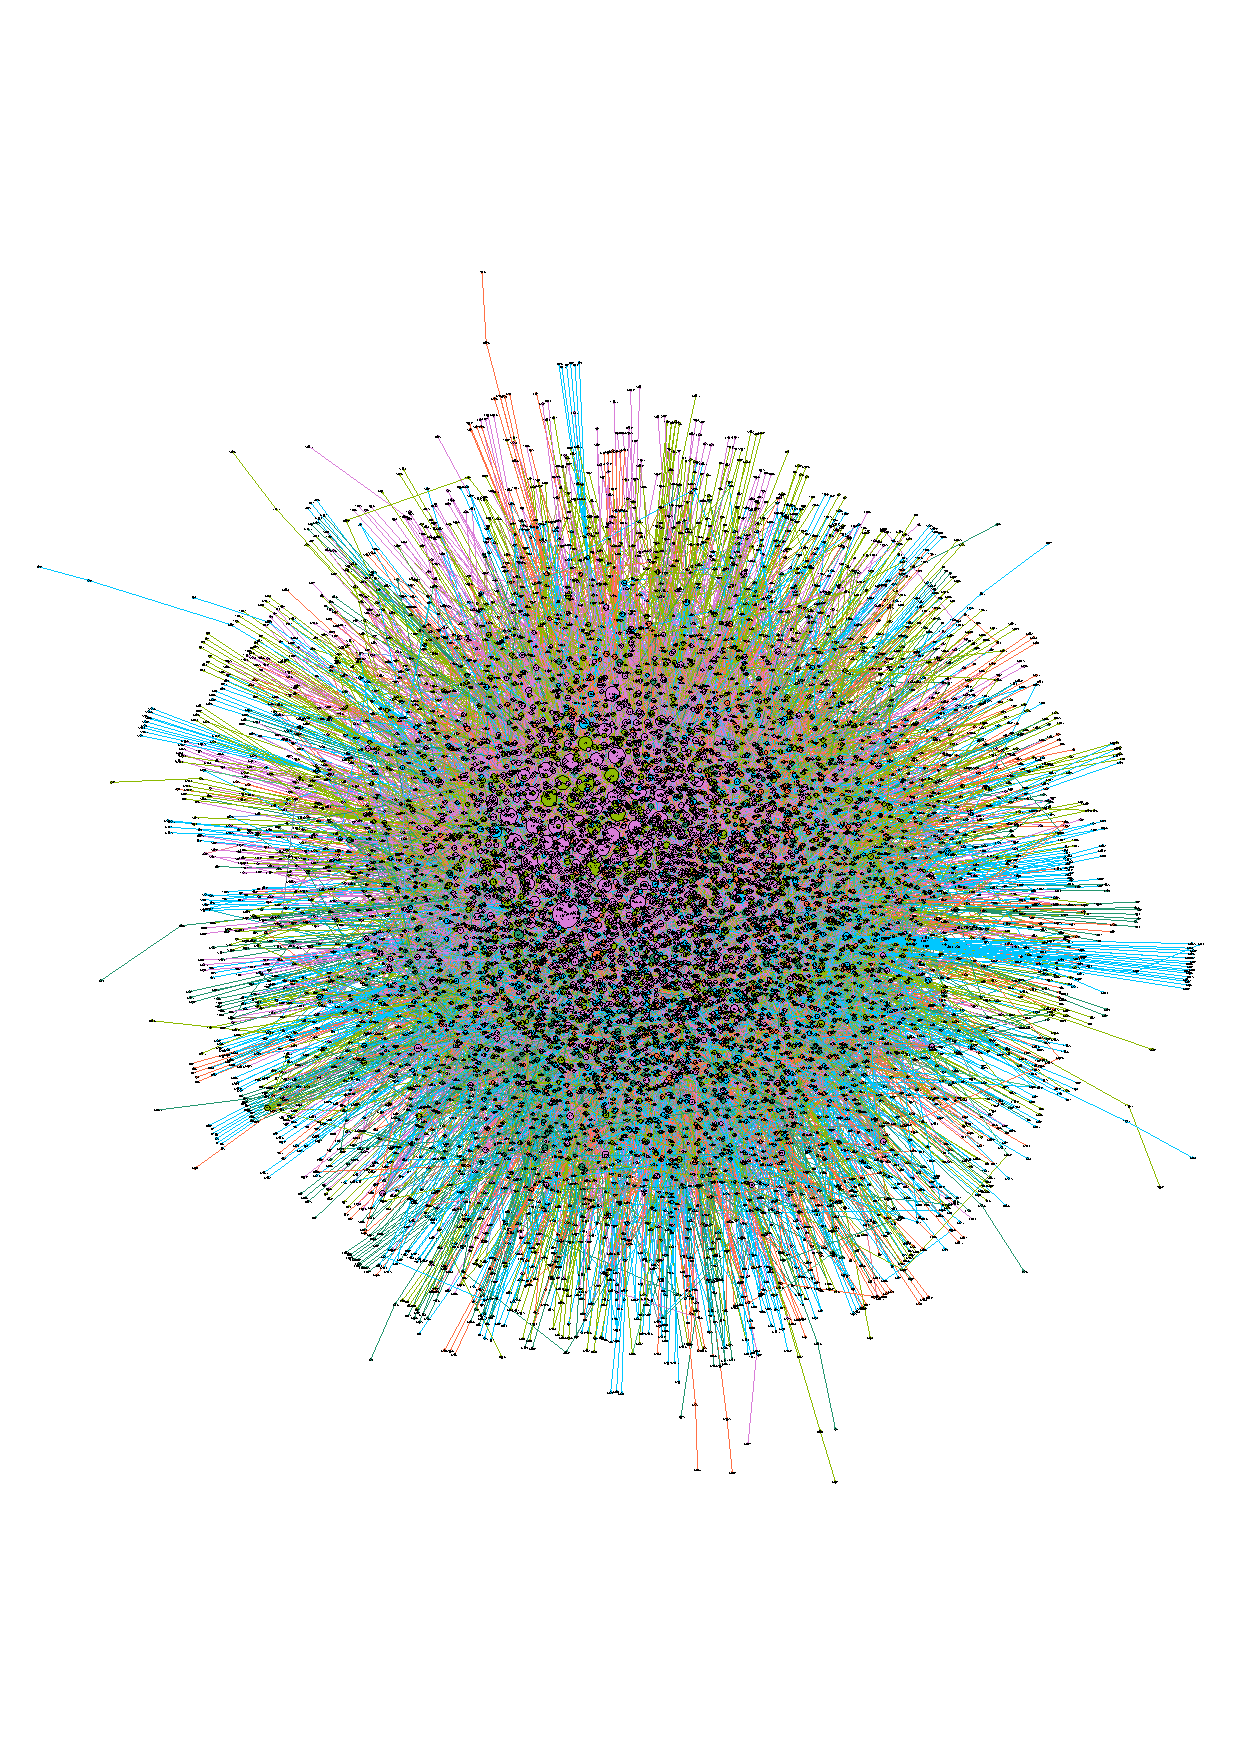
\includegraphics[width=1\textwidth]{export.pdf}
    \caption{Znázornění kompletní sítě}
    \label{network:full}
\end{figure}

\section{Statistiky}
K analýze sítě byl použit nástroj Gephi. Jelikož síť obsahuje velké množství uzlů, těžce se z ní na první pohled dá vyčíst něco zajímavého.
Proto jsem si uzly vyfiltroval podle stupňě uzlů > 17. Toto lze vidět na obrázku \ref{network:filtered}, kde velikost uzlů zachycuje velikost jejich stupně
a barevné obarvení príslušnost do určité komunity.
Distribuce stupňů lze vidět na obrázcích \ref{distribution:degree}, \ref{distribution:in-degree} a \ref{distribution:out-degree}. Jak jde vidět, distribuce
odpovídá spíše mocninnému rozdělení, kde je vysoký počet uzlů s nízkým stupněm a pár uzlů s vysokým stupněm.

Z tohoto už můžeme vyčítat informace. Uzly s vyšším stupněm budou pro tuto síť znamenat pravděpodobně důležitá úložiště, která obsahují buďto velké množství souborů
nebo soubory, o které je velký zájem. Mohou to být převážně nějaké větší servery, zatímco uzly s nizkým stupněm mohou představovat účastníky, kteří síť využívají
spíš pro své vlastní potřeby a stahují soubory.

Průměr sítě, jestliže zanedbáme orientaci hran, čítá 10 uzlů. Průměrná délka cesty je však 4,572. To znamená, že pokud se účastník sítě chce podívat na nějaký sdílený soubor,
jeho požadavek půjde v průměru přes 4 až 5 dalších zařízení v síti. Síť tvoří jedna velká komponenta. I když síť tvoří několik tisíc uzlů, jedná se o 
velice řídkou síť, hustota vychází na minimální 0,001.

Distribuci velikosti komunit zobrazuje obrázek \ref{communities}. V této síti toto může znamenat účastníky v síti, kteří si navzájem sdílí soubory, případně mají
mají vzájemné připojení a navzájem se preferují, jako zdroj dat. Tato lze lépe pozorovat na obrázku \ref{communities:graph}, kde teplota barvy reprezentuje velikost
shlukovacího koeficientu.
Průměrný shlukovací koeficient uzlů je taktéž velmi nízky (0,009), takže žádné velké shluky v síti nelze pozorovat, to je viditelné na obrázku \ref{clustering}.
Absence shluků napovídá tomu, že se skutečně jedná o síť typu P2P a nejsou zde nějaké centrální prvky, na kterých síť stojí, ale vše je sdíleno.

Centrality jsou viditelné na obrázku \ref{centralities}, kde velikost uzlů odpovídá betweeness centralitám a barva
(červená = vysoká centralia, zelená = střední centralita, modrá = nízka) closeness centralitám. Pozorovat můžeme zajívamý uzel uprostřeď sítě, který má
jak vysokou closeness tak betweeness centralitu. Toto bude nějakým způsobem důležitý uzel v síti (např. datové centrum zapojené do této sítě).

\begin{figure}
    \centering
    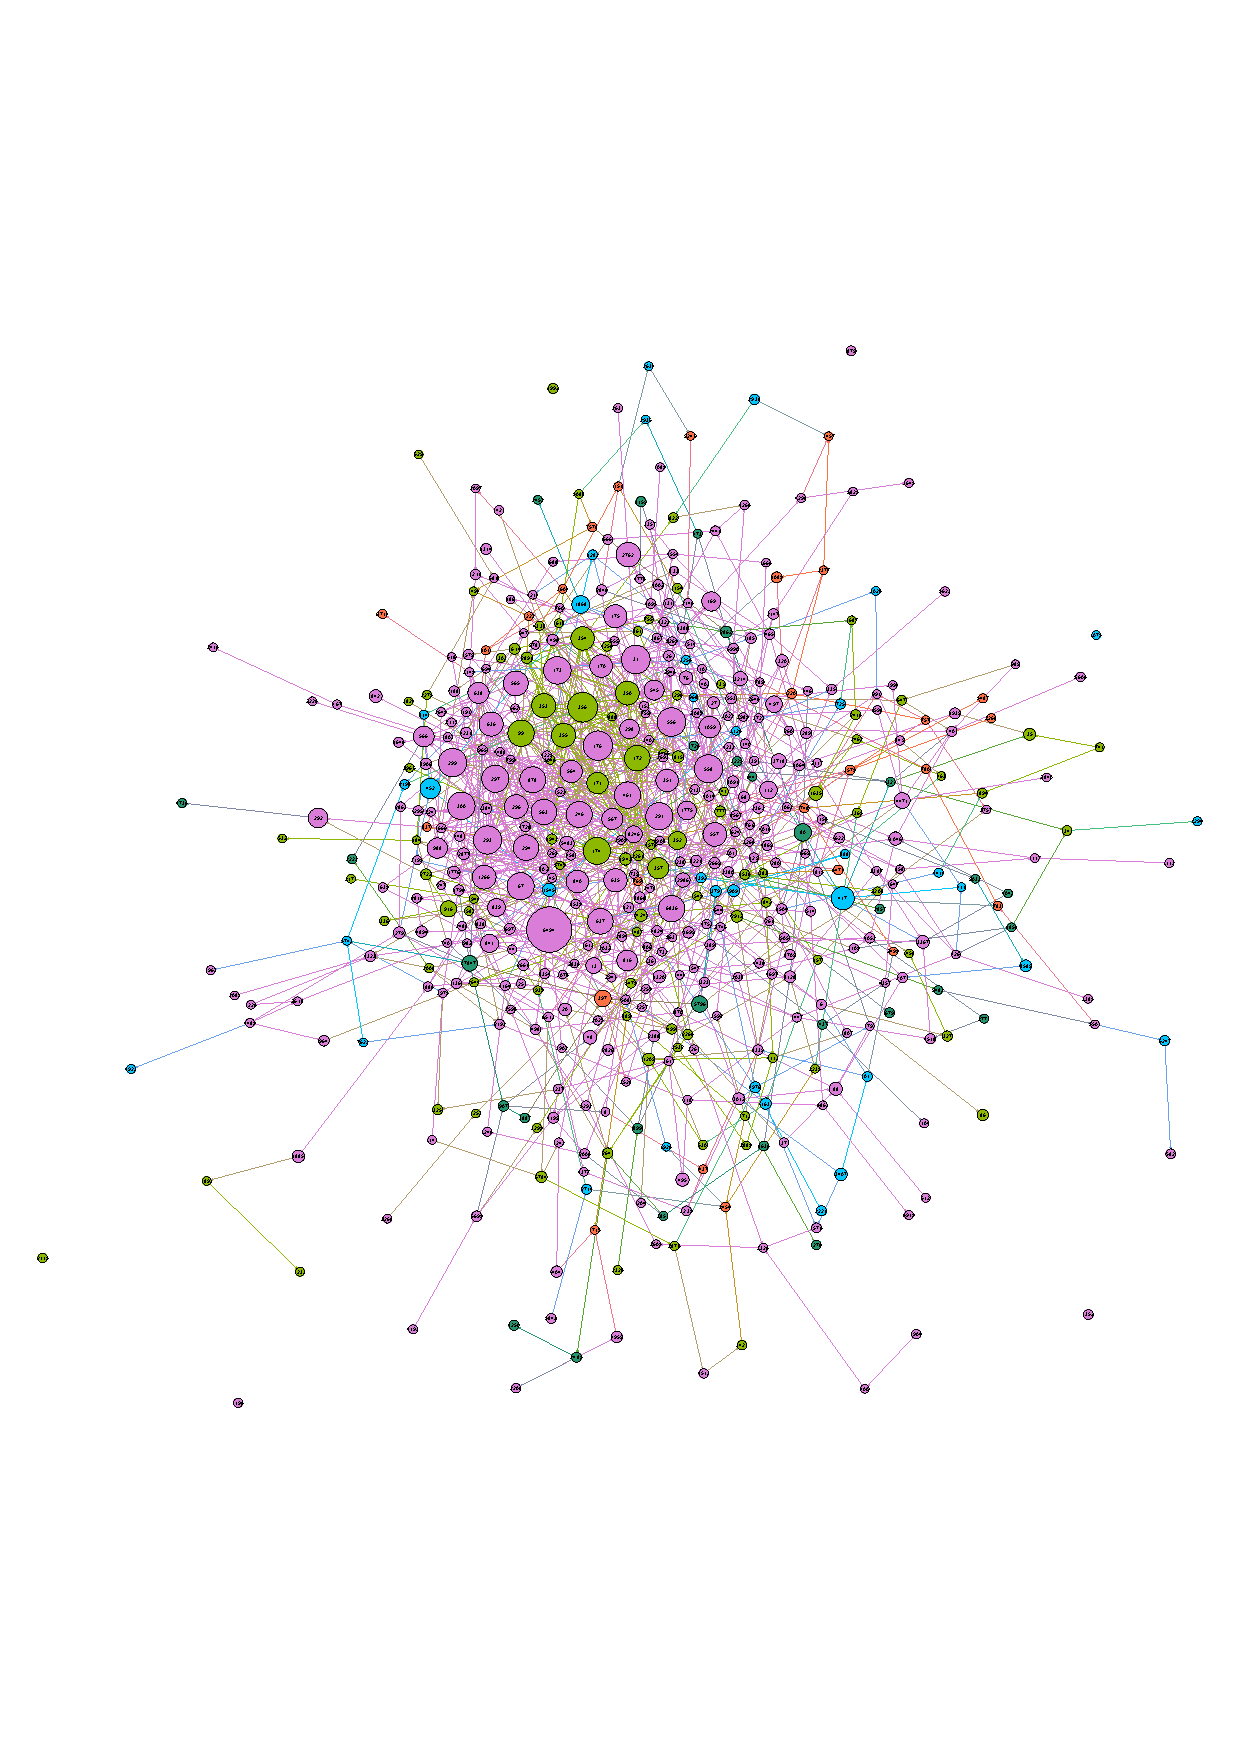
\includegraphics[width=1\textwidth]{export-filtered.pdf}
    \caption{Síť s bez uzlů se stupněm nižším než 17}
    \label{network:filtered}
\end{figure}

\begin{figure}
    \centering
    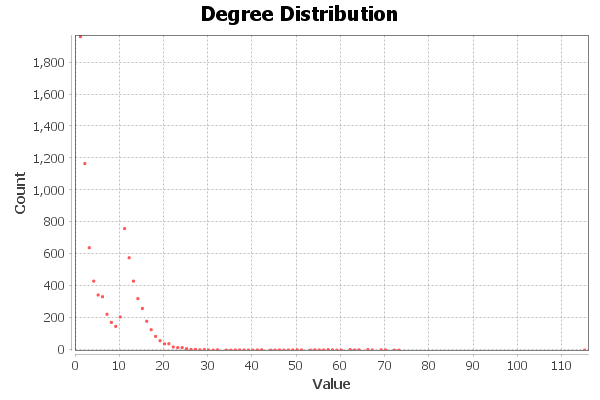
\includegraphics[width=1\textwidth]{degree-report/degree-distribution.png}
    \caption{Distribuce uzlů podle stupně}
    \label{distribution:degree}
\end{figure}

\begin{figure}
    \centering
    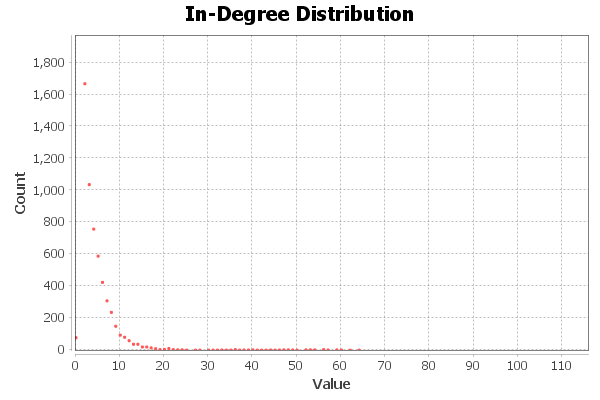
\includegraphics[width=1\textwidth]{degree-report/indegree-distribution.png}
    \caption{Distribuce uzlů podle stupně vstupních hran}
    \label{distribution:in-degree}
\end{figure}

\begin{figure}
    \centering
    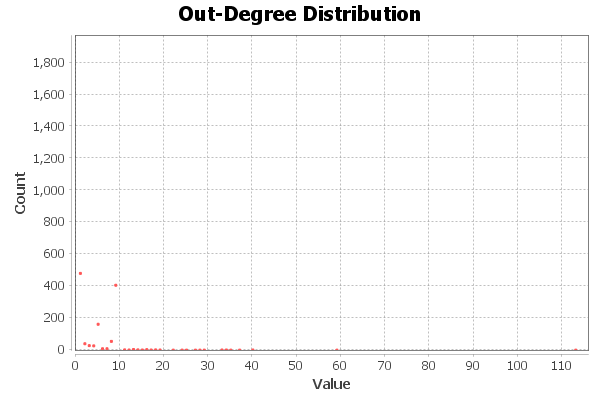
\includegraphics[width=1\textwidth]{degree-report/outdegree-distribution.png}
    \caption{Distribuce uzlů podle stupně odchozích hran}
    \label{distribution:out-degree}
\end{figure}

\begin{figure}
    \centering
    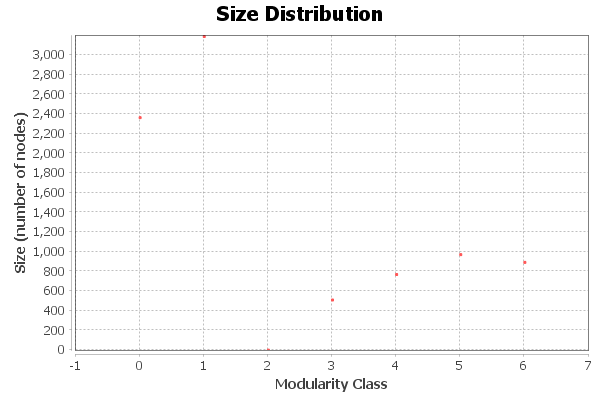
\includegraphics[width=1\textwidth]{modularity/sizes-of-modularities/communities-size-distribution.png}
    \caption{Distribuce velikosti komunit}
    \label{communities}
\end{figure}

\begin{figure}
    \centering
    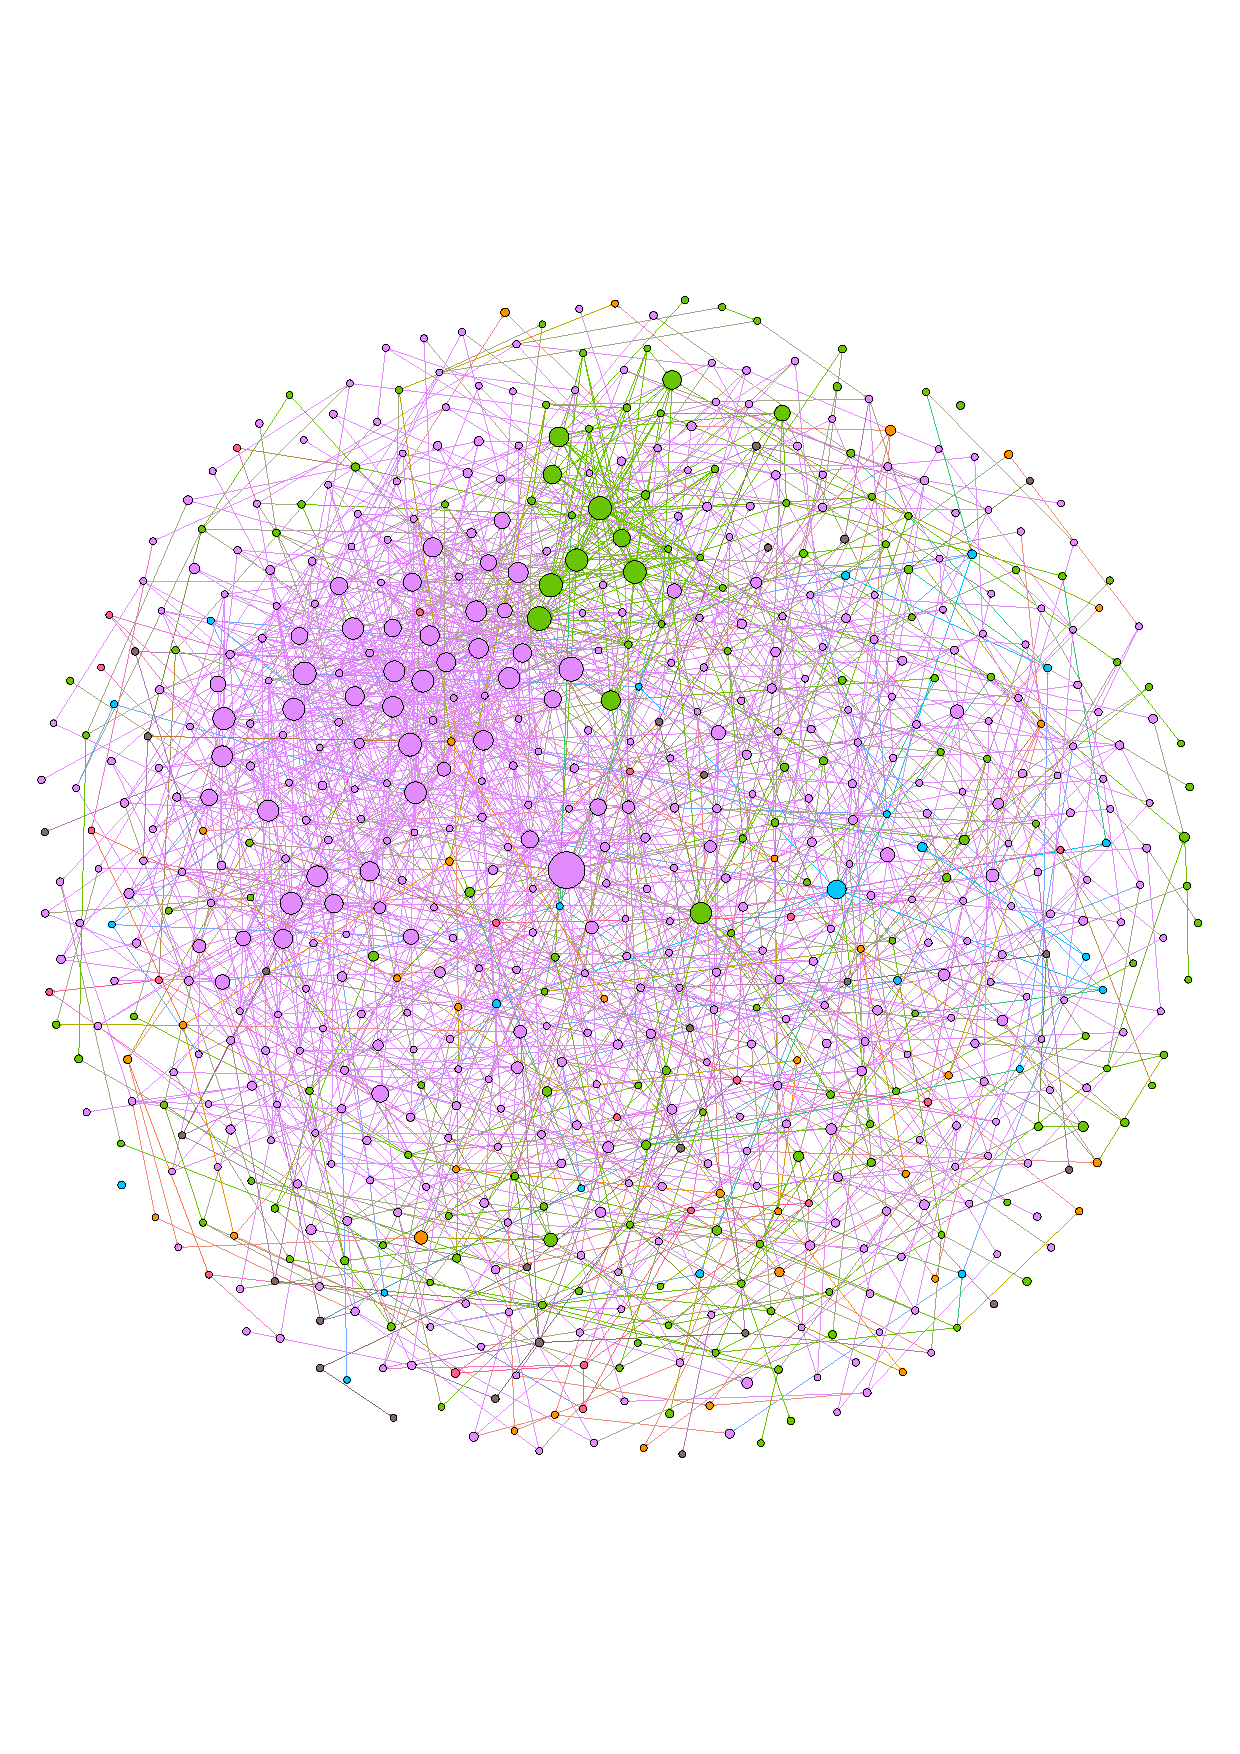
\includegraphics[width=1\textwidth]{communities.pdf}
    \caption{Komunity sítě Gnutella}
    \label{communities:graph}
\end{figure}

\begin{figure}
    \centering
    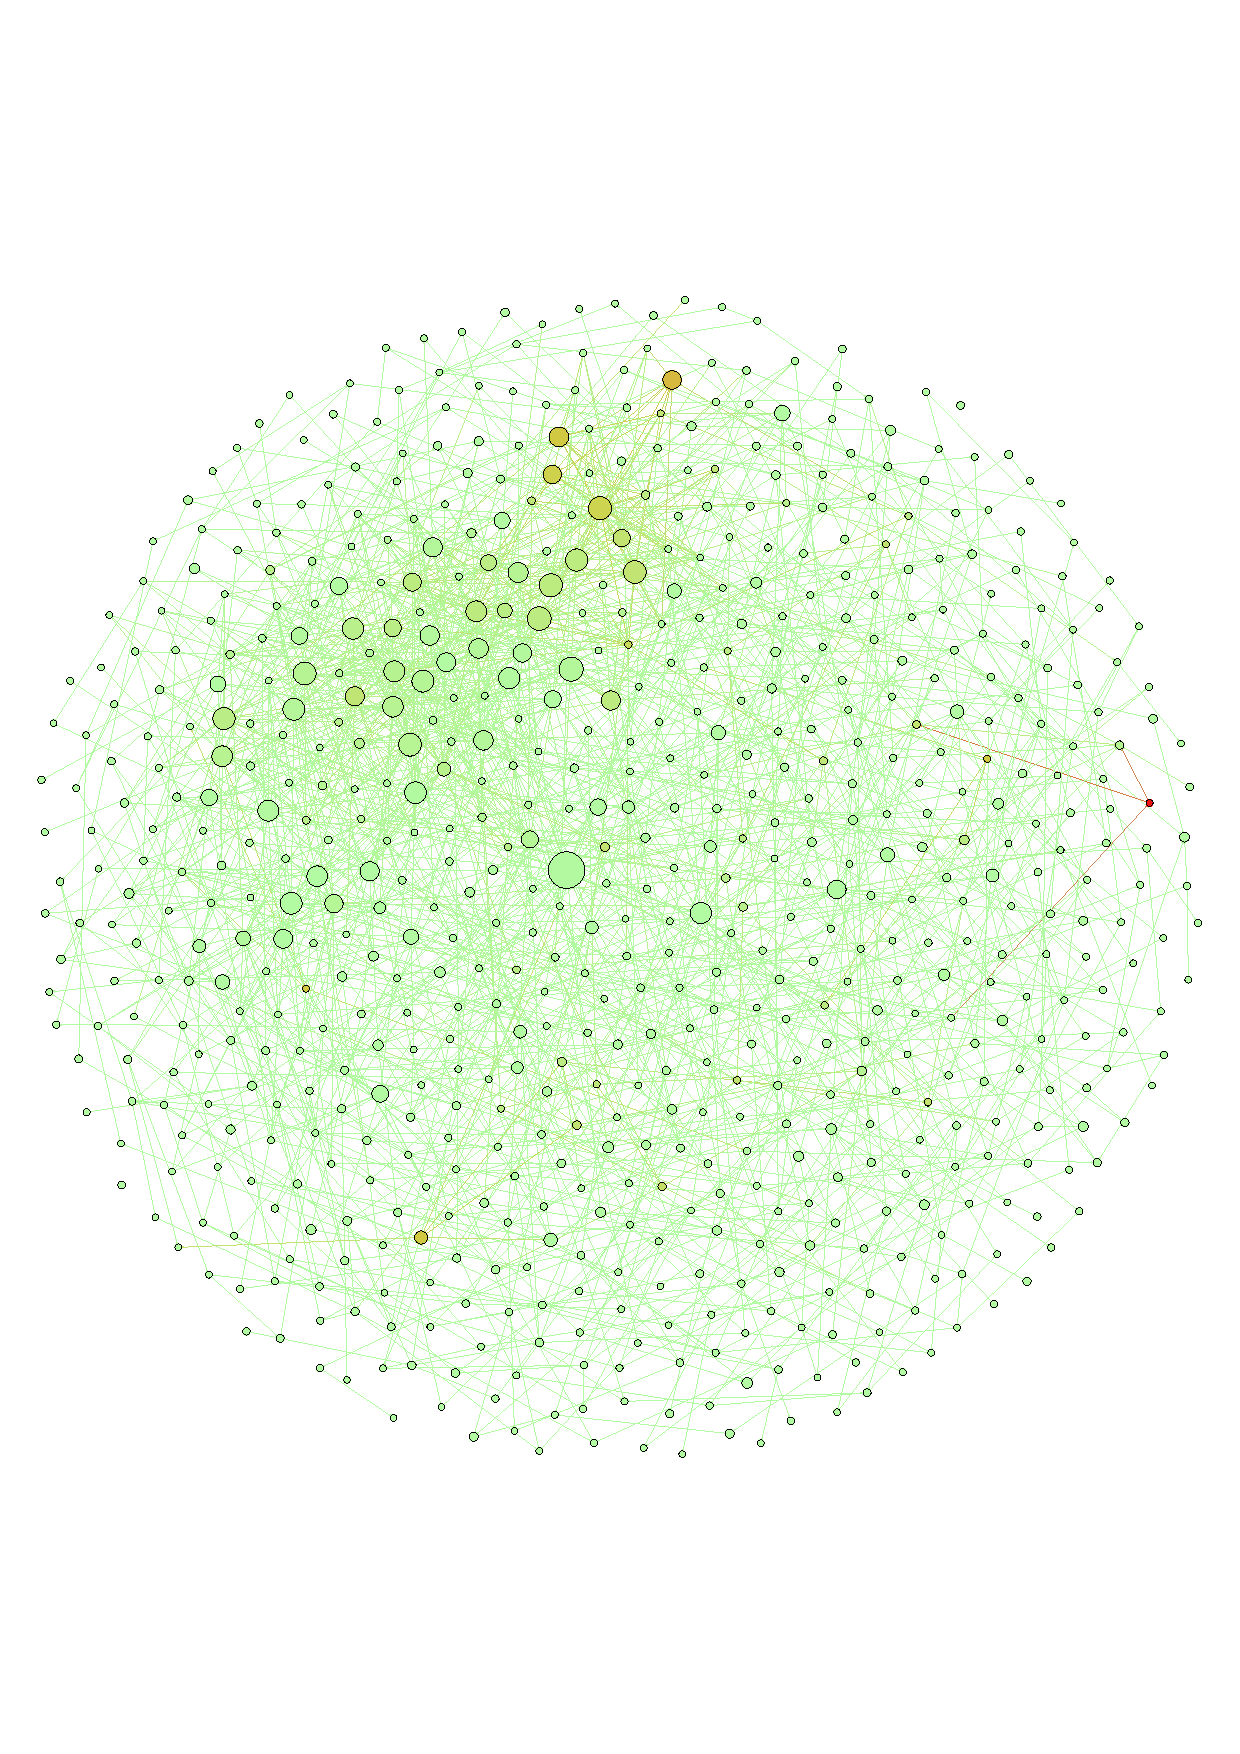
\includegraphics[width=1\textwidth]{clustering-coefficient-ranking.pdf}
    \caption{Shlukovací koeficienty uzlů sítě Gnutella (zelená = nejnižší, červená = nejvyšší)}
    \label{clustering}
\end{figure}

\begin{figure}
    \centering
    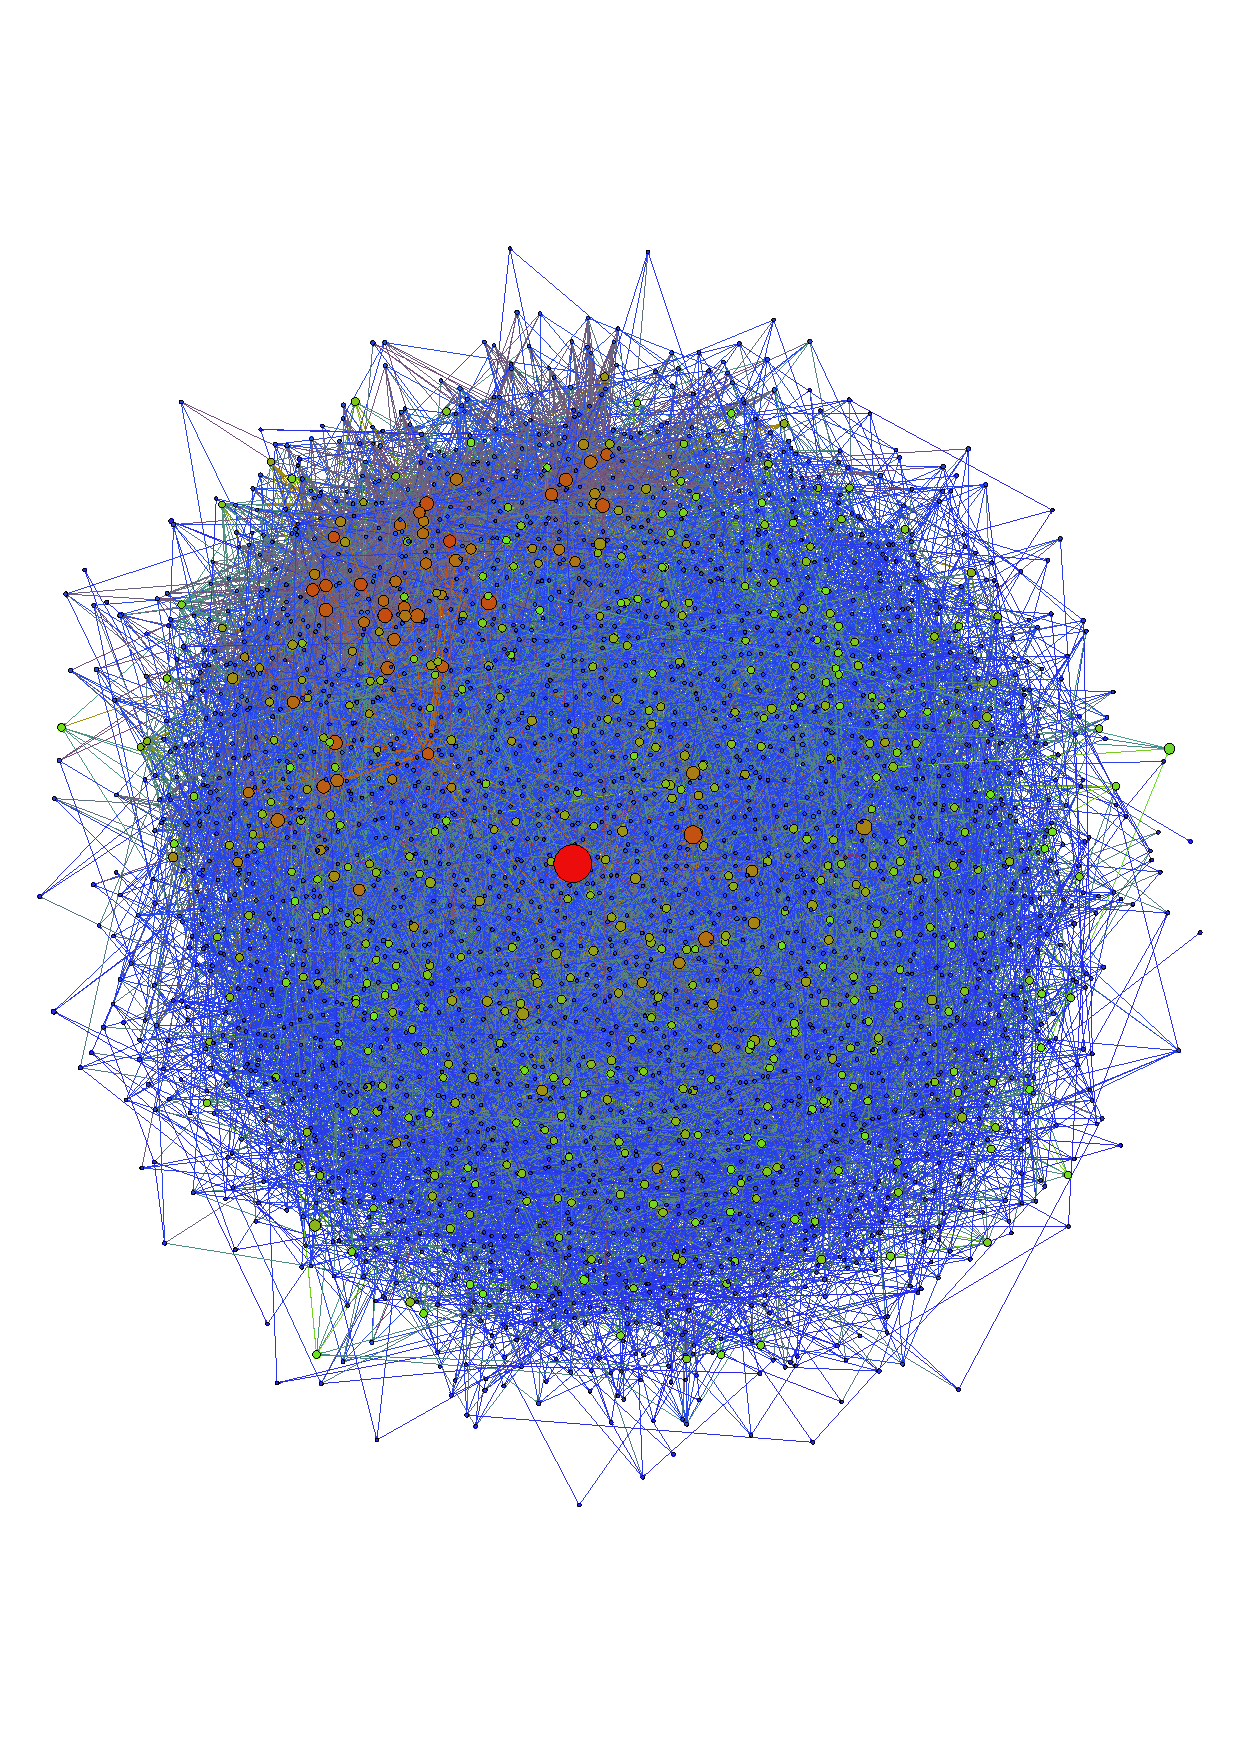
\includegraphics[width=1\textwidth]{centralities.pdf}
    \caption{Centrality, velikost uzlů = betweeness, barva = closeness}
    \label{centralities}
\end{figure}

\clearpage
% Seznam literatury
\printbibliography[title={Literatura}, heading=bibintoc]
\end{document}
